\documentclass[aspectratio=169,xcolor={dvipsnames}]{beamer}

\mode<presentation>
{
  \usetheme{default}
  \usefonttheme{serif}
}
\addtobeamertemplate{navigation symbols}{}{
    \usebeamerfont{footline}
    \usebeamercolor[fg]{footline}
    \hspace{1em}
    \insertframenumber/\inserttotalframenumber
}
\usepackage{minted}
\usepackage{listings}
\usepackage{graphicx}
\usepackage{amsmath,amsthm,amssymb, mathtools}
\usepackage[utf8]{inputenc}
\usepackage{alltt}
\usepackage{xspace}
\usepackage{stmaryrd}
\usepackage{cancel}
\usepackage{palatino,mathpazo}
\usepackage{wasysym}
\usepackage{tikz}
\usepackage{tikz-cd}
\usepackage{multirow}
\usepackage{hyperref}
\usepackage{ebproof}
\usepackage{xcolor}
\usepackage{textcomp}
\usepackage[]{fdsymbol}
\usepackage{multicol}

\definecolor{lightgrey}{RGB}{240,240,240}

\lstdefinelanguage{Lambdapi}
{
  inputencoding=utf8,
  extendedchars=true,
  numbers=none,
  numberstyle={},
  tabsize=2,
  basicstyle={\ttfamily\small\upshape},
%   backgroundcolor=\color{lightgrey},
  keywords={abort,admit,admitted,apply,as,assert,assertnot,associative,assume,begin,builtin,commutative,compute,constant,debug,end,fail,flag,focus,generalize,have,in,induction,inductive,infix,injective,left,let,notation,off,on,opaque,open,prefix,print,private,proofterm,protected,prover,prover_timeout,quantifier,refine,reflexivity,require,rewrite,right,rule,sequential,simplify,solve,symbol,symmetry,type,TYPE,unif_rule,verbose,why3,with},
  sensitive=true,
  keywordstyle=\bfseries\color{blue},
  morecomment=[l]{//},
  morecomment=[n]{/*}{*/},
  commentstyle={\itshape\color{red}},
  string=[b]{"},
  stringstyle=\color{orange},
  showstringspaces=false,
  literate=
  {λ}{$\lambda$}1
  {↪}{$\hookrightarrow$}2
  {→}{$\rightarrow$}2
  {Π}{$\Pi$}1
  {≔}{$\coloneqq$}1
  {⊢}{$\vdash$}1
  {≡}{$\equiv$}1
  {𝔹}{$\mathbb{B}$}1
  {𝕃}{$\mathbb{L}$}1
  {ℕ}{$\mathbb{N}$}1
  {α}{$\alpha$}1
  {β}{$\beta$}1
  {η}{$\eta$}1
  {π}{$\pi$}1
  {τ}{$\tau$}1
  {ω}{$\omega$}1
  {∧}{$\wedge$}1
  {≤}{$\le$}1
  {≠}{$\neq$}1
  {∉}{$\notin$}1
  {×}{$\times$}1
  {⋅}{$\cdot$}1
  {⟇}{$\veedot$}1
  {□}{$\Square$}1
  {⊤}{$\top$}1
  {π̇}{$\dot{\pi}$}1
  {φ₁}{$\varphi_1$}1
  {ₙ}{$_n$}1
  {ₖ}{$_k$}1
  {π}{$\pi$}1
}
\lstset{
    language=Lambdapi,
}

\definecolor{darkgray}{rgb}{.4,.4,.4}

\lstset{
    aboveskip={1.3\baselineskip},
    basicstyle=\footnotesize\ttfamily\linespread{4},
    breaklines=false,
    columns=fixed,
    commentstyle=\color[rgb]{0.127,0.427,0.514}\ttfamily\itshape,
    escapechar=@,
    extendedchars=true,
    frame=single,
    identifierstyle=\color{black},
    inputencoding=latin1,
    language=Lambdapi,
    numbers=left,
    numberstyle=\tiny,
    prebreak = \raisebox{0ex}[0ex][0ex]{\ensuremath{\hookleftarrow}},
    stringstyle=\color[rgb]{0.639,0.082,0.082}\ttfamily,
    upquote=true,
    showstringspaces=false
}

\hypersetup{
    linkcolor=blue,
    urlcolor=cyan,
    pdftitle={Overleaf Example},
    pdfpagemode=FullScreen,
}

\newcommand*\circled[1]{\tikz[baseline=(char.base)]{
            \node[shape=circle,draw,inner sep=2pt] (char) {#1};}}


\def\nstarlexer{lexer/nstar.py:NStarLexer -x}

\usetikzlibrary{positioning,shapes,shapes.symbols,fit,shadows,arrows}
\usetikzlibrary{arrows,chains,matrix,scopes}

\def\imp{\rightarrow}

\makeatletter

\tikzset{
  shift left/.style ={commutative diagrams/shift left={#1}},
  shift right/.style={commutative diagrams/shift right={#1}}
}

\lstset{
    escapeinside={(@}{@)},          % if you want to add LaTeX within your code
}


\usepackage{tlaps}

\def\checkmark{\tikz\fill[scale=0.4](0,.35) -- (.25,0) -- (1,.7) -- (.25,.15) -- cycle;} 

\title{Reconstruction of TLAPS proofs\\ solved by SMT in Lambdapi}

\author[A.~Colt]{%
  Alessio Coltellacci
}
\institute[]{\small%
  Univ. Lorraine, CNRS, Inria, Loria
}

\date[]{%
  ICSPA
}

\AtBeginSubsection[]{%
  \begin{frame}%<beamer>
    \frametitle{Outline}
    \small
    \tableofcontents[sectionstyle=show/shaded,subsectionstyle=show/shaded/hide]
  \end{frame}
}

\newcommand\chighlight[2]{\setlength{\fboxsep}{0pt}\colorbox{#1}{#2\strut}}

\makeatletter
\newcommand{\minted@addto@optlistclswitch}[2]{%
  \expandafter\def\expandafter#1\expandafter{#1%
    \detokenize{#2}\space}}
\newcommand{\minted@addto@optlistcl@langswitch}[2]{%
  \expandafter\let\expandafter\minted@tmp\csname #1\endcsname
  \expandafter\def\expandafter\minted@tmp\expandafter{\minted@tmp%
    \detokenize{#2}\space}%
  \expandafter\let\csname #1\endcsname\minted@tmp}
\newcommand{\minted@def@optcl@filterswitch}[2]{%
  \define@booleankey{minted@opt@g}{#1}%
  {\minted@addto@optlistclswitch{\minted@optlistcl@g}{#2}{}%
    \@namedef{minted@opt@g:#1}{true}}
  {\minted@addto@optlistclswitch{\minted@optlistcl@g}{}{}%
    \@namedef{minted@opt@g:#1}{false}}
  \define@booleankey{minted@opt@g@i}{#1}%
  {\minted@addto@optlistclswitch{\minted@optlistcl@g@i}{#2}{}%
    \@namedef{minted@opt@g@i:#1}{true}}
  {\minted@addto@optlistclswitch{\minted@optlistcl@g@i}{}{}%
    \@namedef{minted@opt@g@i:#1}{false}}
  \define@booleankey{minted@opt@lang}{#1}%
  {\minted@addto@optlistcl@langswitch{minted@optlistcl@lang\minted@lang}{#2}{}%
    \@namedef{minted@opt@lang\minted@lang:#1}{true}}
  {\minted@addto@optlistcl@langswitch{minted@optlistcl@lang\minted@lang}{}{}%
    \@namedef{minted@opt@lang\minted@lang:#1}{false}}
  \define@booleankey{minted@opt@lang@i}{#1}%
  {\minted@addto@optlistcl@langswitch{minted@optlistcl@lang\minted@lang@i}{#2}{}%
    \@namedef{minted@opt@lang\minted@lang@i:#1}{true}}
  {\minted@addto@optlistcl@langswitch{minted@optlistcl@lang\minted@lang@i}{}{}%
    \@namedef{minted@opt@lang\minted@lang@i:#1}{false}}
  \define@booleankey{minted@opt@cmd}{#1}%
  {\minted@addto@optlistclswitch{\minted@optlistcl@cmd}{#2}{}%
    \@namedef{minted@opt@cmd:#1}{true}}
  {\minted@addto@optlistclswitch{\minted@optlistcl@cmd}{}{}%
    \@namedef{minted@opt@cmd:#1}{false}}
}
\minted@def@optcl@filterswitch{allowlocal}{-x}
\makeatother
\setminted{allowlocal}

\begin{document}

\begin{frame}
  \titlepage
  \centering
    \begin{minipage}{.18\textwidth}
        
\includegraphics[width=2.5cm]{ul_logo.png}
    \end{minipage}%
    \begin{minipage}{.12\textwidth}
        
\includegraphics[width=1.5cm]{cnrs.png}
    \end{minipage}%
    \begin{minipage}{.18\textwidth}
        
\includegraphics[width=2.5cm]{inria-logo.png}
    \end{minipage}%
    \begin{minipage}{.12\textwidth}
        
\includegraphics[width=1.5cm]{loria-logo.png}
    \end{minipage}%
    % \hspace{\stretch{1}}%
\end{frame}

\begin{frame}{Outline}
    \tableofcontents
\end{frame}

\section{SMT translation at a glance}

\AtBeginSection[]
{
  \begin{frame}
    \tableofcontents[currentsection]
  \end{frame}
}

\begin{frame}{\tlaplus at a glance}
\begin{columns}[T] % align columns
    \begin{column}{.48\textwidth}
    \begin{itemize}
       \o Specification language to design and verify reactive systems
        \o Systems are described as state machines
    \end{itemize}
    \end{column}%
    \begin{column}{.48\textwidth}
    \vbox to .48\textheight{%
        $VARIABLE~x$\\
        $CONSTANT~N$ \\
        $ASSUME~N \in Nat$

         \vfill
    
        $\begin{noj}
        Init \deq \quad\begin{conj}
              x = 0
        \end{conj}
        \end{noj}$
        
        \vfill
       
        $\begin{noj}
        Next \deq \quad\begin{conj}
            x < N \\
            x' = x + 1
        \end{conj}
        \end{noj}$

        \vfill

        $Spec \deq Init \land  \square [Next]_{\seq{x}}$
    }%
    \end{column}%
\end{columns}
\end{frame}

\begin{frame}{TLAPS proof example}
\begin{math}
--------------\text{MODULE Cantor1}-----------------\\
\THEOREM~~\text{cantor}~~== \\
~\qquad\A ~S~:\\
~\qquad\qquad\A~f \in [ S \rightarrow \SUBSET~S ]~:\\
~\qquad\qquad\qquad\E~A \in \SUBSET~S~: \\
~\qquad\qquad\qquad\qquad\A~x \in S~: \\
~\qquad\qquad\qquad\qquad \quad f~[x] ~\#~ A~\\
\PROOF\\
<\!1\!>1. \quad \TAKE~S \\
<\!1\!>2. \quad \TAKE ~f \in [S \rightarrow \SUBSET~S] \\
<\!1\!>3. \quad \DEFINE ~T~ == \{~z \in S ~:~ z \notin f[z]~\} \\
<\!1\!>4. \quad \WITNESS ~T \in \SUBSET~S\\
<\!1\!>5. \quad \TAKE~x \in S\\
<\!1\!>6. \quad \QED~\BY~x \in T \lor x \notin T\\
\end{math}
\end{frame}


\begin{frame}{Proposed solution}
    \begin{figure}
    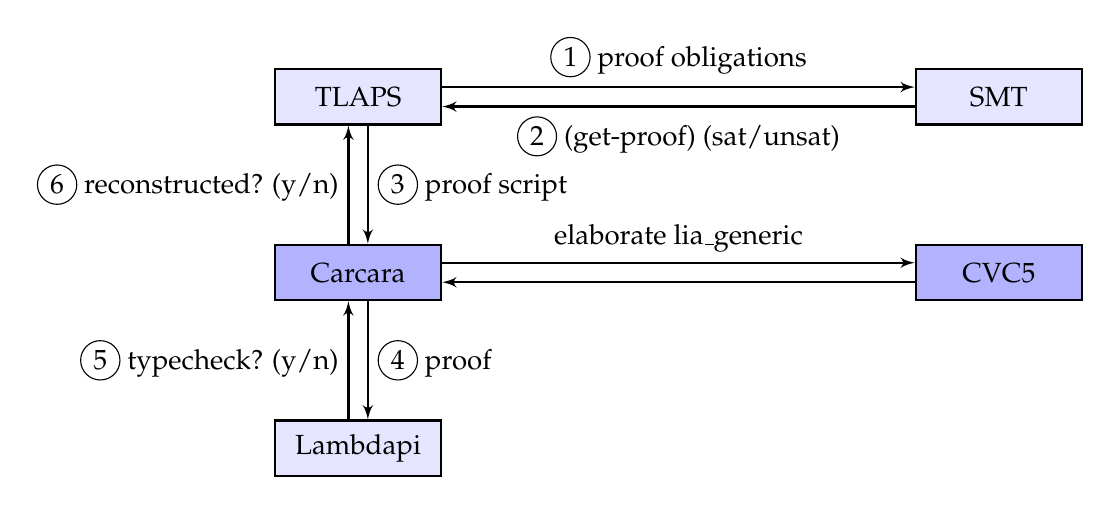
\begin{tikzpicture}[
      node distance=1.5cm and 6cm,
      >=latex',
      auto,
      thick,
      service/.style={draw, fill=blue!10,  minimum height=2em, minimum width=6em},
      newservice/.style={draw, fill=blue!30,  minimum height=2em, minimum width=6em},
    ]
      \node[service] (tlaps) {TLAPS};
      \node[service, right = of tlaps] (smt) {SMT};
      \node[newservice, below = of tlaps] (recon) {Carcara};
      \node[newservice, right = of recon] (zenon) {CVC5};
      \node[service, below = of recon] (lm) {Lambdapi};
    
    \path[->, shift left=.75ex]
        (tlaps) edge node {\circled{1} proof obligations}   (smt)
        (smt) edge   node {\circled{2} (get-proof) (sat/unsat)} (tlaps)
        (tlaps) edge node {\circled{3} proof script} (recon)
        (recon) edge node {\circled{6} reconstructed? (y/n)}   (tlaps)
        (recon) edge  node {\circled{4} proof} (lm)
        (lm) edge  node {\circled{5} typecheck? (y/n)} (recon)
        (recon) edge node {elaborate lia\_generic}   (zenon)
        (zenon) edge node {}   (recon);
      \end{tikzpicture}
    \end{figure}
\end{frame}

\begin{frame}[fragile]{Simple example}
    \begin{minted}[allowlocal,autogobble, fontsize=\footnotesize, frame=single]{smt.py:CustomLexer}
        (set-logic QF_UF)
        (declare-sort U 0)
        (declare-fun a () U)
        (declare-fun b () U)
        (declare-fun p (U) Bool)
        (assert (p a))
        (assert (= a b))
        (assert (not (p b)))
        (get-proof)
    \end{minted}
\end{frame}

\begin{frame}[fragile]{Its Alethe SMT proof}
    \begin{minted}[allowlocal,autogobble, fontsize=\footnotesize, frame=single]{smt.py:CustomLexer}
        (assume a0 (p a))
        (assume a1 (= a b))
        (assume a2 (not (p b)))
        (step t1 (cl (not (= (p a) (p b))) (not (p a)) (p b)) :rule equiv_pos2)
        (step t2 (cl (= (p a) (p b))) :rule cong :premises (a1))
        (step t3 (cl (p b)) :rule resolution :premises (t1 t2 a0))
        (step t4 (cl) :rule resolution :premises (a2 t3))
    \end{minted}
\end{frame}


\begin{frame}{Alethe format}
\begin{definition}[Alethe step]
A proof in the Alethe language is an indexed list of step following the format:
\begin{equation*}
    j. \quad  \Delta \quad \vdash~ \varphi \quad (R; p_1 \dots p_n)[a_1, \dots, a_n]\quad
\end{equation*}
\begin{itemize}
    \item[] With $i \in \mathbb{I}$  where $\mathbb{I}$ is a countable infinite set of valid indices, 
    \item[] a formula $\varphi$,
    \item[] a rule name $\mathcal{R}$ from a set of possible rules,
    \item[] a possible empty sets $\{ p_1 \dots p_n \} \subseteq \mathbb{I}$ of premises (previous steps),
    \item[] a possible empty list of arguments $[a_1 \dots a_n]$ where $a_i = (x_i, t_i)$\\
    with $x_i$ a variable and $t_i$ a term,
    \item[] and a context $\Delta$.
\end{itemize}
\end{definition}
\end{frame}

\begin{frame}[t]{Overview of rules}
\begin{multicols}{2}
    \begin{enumerate}
        \item Special rules
        \begin{itemize}
            \item[*] \textsubscript{$\vdash~\varphi\quad\texttt{(asssume)}$}
            \item[*] \textsubscript{$\vdash~\varphi\quad(\texttt{hole};~p_1 \dots p_n)[a_1\dots a_n]$}
            \item[*] \textsubscript{$\varphi_1 \dots \varphi_n,~\psi~\vdash~ \neg \varphi_1 \dots \neg \varphi_n \psi$}
                    \textsubscript{$\qquad\qquad (\texttt{subproof};~p_1 \dots p_n)$}
        \end{itemize}
        \item Resolution rules
        \begin{itemize}
            \item[*] \textsubscript{$\texttt{th\_resolution,resolution}$}
            \item[*] \textsubscript{$\texttt{contraction},~\texttt{reordering}$}
        \end{itemize}
        \item Introducing tautologies
        \begin{itemize}
            \item[*] \textsubscript{$\vdash~ \neg (\neg\neg\varphi),~\varphi \quad\texttt{(not\_not)}$}
            \item[*] \textsubscript{$\vdash~ \neg (\varphi_1 \approx \varphi_2),~ \neg \varphi_1,~\varphi_2  \quad\texttt{(equiv\_pos2)}$}
            \item[*] \textsubscript{$\vdash~ \neg (\varphi_1 \land \dots \land \varphi_n),~\varphi_k \quad\texttt{(and\_pos)}$}
        \end{itemize}
        \item Linear arithmetic
        \begin{itemize}
            \item[*] \textsubscript{$\texttt{lia\_generic,la\_generic}$}
            \item[*] \textsubscript{$\vdash~ t_1 \leq t_2 \lor t_2 \leq t_1 \texttt{(la\_totality)}$}
        \end{itemize}
        \item Quantifier handling
        \begin{itemize}
            \item[*] \textsubscript{$j.~\Delta,~x_i \mapsto y_i \vdash~ \varphi \approx \varphi'$}
                \newline \textsubscript{$i. \vdash  \forall x_1 \dots x_n, \varphi \approx \forall y_1 \dots y_n, \varphi' ~\texttt{(bind)}$}
            \item[*] \textsubscript{$\texttt{forall\_inst}$}
        \end{itemize}
        \item Skolemization
        \begin{itemize}
            \item[*] \textsubscript{$\texttt{sko\_ex}$}
            \item[*] \textsubscript{$\texttt{sko\_forall}$}
        \end{itemize}
        \item Clausification rules
        \begin{itemize}
            \item[*] \textsubscript{$\textbf{let}$}
            \item[*] \textsubscript{$\texttt{distinct\_elim}$}
        \end{itemize}
        
        \item Simplification rules
        \begin{itemize}
            \item[*] \textsubscript{$\texttt{and\_simplify}$}
            \item[*] \textsubscript{$\texttt{bool\_simplify}$}
            \item[*] \textsubscript{$\texttt{eq\_simplify}$}
            \item[*] \textsubscript{$\texttt{sum\_simplify}$}
        \end{itemize}
    \end{enumerate}
\end{multicols}
\end{frame}
    

\begin{frame}[fragile]{Alethe proof as derivation tree}
        \begin{center}
        \begin{prooftree}
            \hypo{}
            \ellipsis{}{}
            \infer[left label=$t_j$]1[\footnotesize Rule(\dots)]{\Delta'' \vdash p_1}
            \hypo{ \dots }
            \hypo{}
            \ellipsis{}{}
            \infer[left label=$t_k$]1[\footnotesize Rule(\dots)]{\Delta' \vdash p_n}
            \infer[left label=$t_i$]3[\footnotesize Rule($a_1 \dots a_n$)]{ \Delta \cup \{ p_1 \dots p_n \} \vdash c_1, \dots, c_n }
        \end{prooftree}
    \end{center}
\end{frame}

\begin{frame}[fragile]{Loop back on the SMT proof example}
\begin{minted}[allowlocal,autogobble, fontsize=\footnotesize, frame=single]{smt.py:CustomLexer}
    (assume a0 (p a))
    (assume a1 (= a b))
    (assume a2 (not (p b)))
    (step t1 (cl (not (= (p a) (p b))) (not (p a)) (p b)) :rule equiv_pos2)
    (step t2 (cl (= (p a) (p b))) :rule cong :premises (a1))
    (step t3 (cl (p b)) :rule resolution :premises (t1 t2 a0))
    (step t4 (cl) :rule resolution :premises (a2 t3))
\end{minted}
\vfill
This proof can not be reconstructed directly due to coarse-grained steps e.g: pivots are not given for t3 and t4. 
\end{frame}

\begin{frame}{Carcara}
    \begin{itemize}
    \item Carcara is an efficient and independent proof checker and
    elaborator for Alethe proofs.
    \item Carcara is written in Rust, a high performance language,
    \item implements elaboration procedures for a few important rules (ex: infering pivots),
    \item it remove implicit transformations (ex: reordering clause).
    \end{itemize}
\end{frame}


\begin{frame}[fragile]{Elaborated proof with Carcara}
    Make pivot and resolution order explicit\\
    \begin{minted}[allowlocal,autogobble, fontsize=\footnotesize, frame=single, escapeinside=||]{smt.py:CustomLexer}
        (assume a0 (p a))
        (assume a1 (= a b))
        (assume a2 (not (p b)))
        (step t1 (cl (not (= (p a) (p b))) (not (p a)) (p b)) :rule equiv_pos2)
        (step t2 (cl (= (p a) (p b))) :rule cong :premises (a1))
        (step t3 (cl (p b)) :rule resolution :premises (t1 t2 a0)
            |\chighlight{yellow!60}{:args ((= (p a) (p b)) false (p a) false)}|)
        (step t4 (cl) :rule resolution :premises (a2 t3)
            |\chighlight{yellow!60}{:args ((p b) false)}|)
    \end{minted}
\end{frame}



\begin{frame}{Corresponding proof tree}
    \begin{figure}
        \centering
        \resizebox{\textwidth}{!}{
            \begin{prooftree}
                \infer[left label=$a_0$]0{ \Delta ~\vdash~p(a) }
                \infer[left label=$t_1$]0[equiv\_pos2]{ \Delta ~\vdash~\neg~(p(a) = p(b)), \neg p(a), p(b) }
                \infer[left label=$t_2$]0[cong($a_1$)]{ \Delta ~\vdash~ p(a) = p(b) }
                \infer[left label=$t_3'$]2[Resolution($t_1$, $t_2$) ]{ \Delta ~\vdash~ \neg p(a), p(b) }
                \infer[left label=$t_3$]2[Resolution($a_0,t3'$)]{ \Delta ~\vdash~p(b) }
                \infer[left label=$a_2$]0{ \Delta ~\vdash~ \neg~p(b) }
                \infer[left label=$t_4$]2[Resolution($a_2, t_3$)]{ \Delta ~\vdash~\bot }
            \end{prooftree}
        }
    \end{figure}
\end{frame}


\begin{frame}[fragile]{Translate prelude}
\noindent\begin{minipage}{.45\textwidth}
\begin{minted}[allowlocal, autogobble, fontsize=\footnotesize, frame=single, linenos]{smt.py:CustomLexer}
(declare-sort U 0)
(declare-fun a () U)
(declare-fun b () U)
(declare-fun p (U) Bool)
\end{minted}
\end{minipage}
$\leadsto$\hfill \begin{minipage}{.45\textwidth}
\begin{lstlisting}[]
symbol U : TYPE;
rule U ↪ τ o;

symbol a : U;
symbol b : U;
symbol p : U → Prop;
\end{lstlisting}
\end{minipage}
\end{frame}

\begin{frame}[fragile]{Translate assert/assume}
\noindent\begin{minipage}{.40\textwidth}
\begin{minted}[allowlocal, autogobble, fontsize=\footnotesize, frame=single, linenos]{smt.py:CustomLexer}
(assert (p a))
(assert (= a b))
(assert (not (p b)))
\end{minted}
\end{minipage}
\newline
\noindent\begin{minipage}{.40\textwidth}
\begin{minted}[allowlocal, autogobble, fontsize=\footnotesize, frame=single, linenos]{smt.py:CustomLexer}
(assume a0 (p a))
(assume a1 (= a b))
(assume a2 (not (p b)))
\end{minted}
\end{minipage}
\hfill\begin{minipage}{.55\textwidth}
\begin{lstlisting}[escapeinside={(*}{*)}]
constant symbol a0 : (*$\dot{\pi}$*) (p a (*$\veedot~\Square$*));
constant symbol a1 :
    (*$\dot{\pi}$*) (a (*$\iff^c$*) b (*$\veedot~\Square$*));
constant symbol a2 :
    (*$\dot{\pi}$*) ((*$\neg^c$*) (p b) (*$\veedot~\Square$*));
\end{lstlisting}
\end{minipage}
\end{frame}

\begin{frame}[fragile]{Translation of step t1 and t2}
\noindent\begin{minipage}{.45\textwidth}
\begin{minted}[allowlocal, autogobble, fontsize=\footnotesize, frame=single, linenos]{smt.py:CustomLexer}
(step t1
    (cl (not (= (p a) (p b)))
        (not (p a))
        (p b))
    :rule equiv_pos2)
(step t2 (cl (= (p a) (p b)))
    :rule cong :premises (a1))
...
\end{minted}
\end{minipage}
$\leadsto$\hfill \begin{minipage}{.45\textwidth}
\begin{lstlisting}[escapeinside={(*}{*)}]
opaque symbol pb : 
begin
have t1: (*$\dot{\pi}$*) (
    (*$\neg^c$*) ((p a) (*$\iff^c$*) (p b))
    (*$\veedot$*) (p a)
    (*$\veedot$*) (p b)
    (*$\veedot~\Square$*))
{
    apply equiv_pos2;
};
have t2: (*$\dot{\pi}$*) (
    p a (*$\iff^c$*) p b
    (*$\veedot~\Square$*))
{
    apply (*$\lor^c_{i1}$*);
    apply cong p a1;
};
\end{lstlisting}
\end{minipage}
\end{frame}

\begin{frame}[fragile]{Translation of step t3}
\noindent\begin{minipage}{.35\textwidth}
\begin{minted}[allowlocal, autogobble, fontsize=\footnotesize, frame=single, linenos]{smt.py:CustomLexer}
(step t3 (cl (p b)) 
    :rule resolution
    :premises (t1 t2 a0))
    :args (
    (= (p a) (p b)) false
    (p a) false
    ))
\end{minted}
\end{minipage}
$\leadsto$\hfill \begin{minipage}{.55\textwidth}
\begin{lstlisting}[escapeinside={(*}{*)}]
...
have t3 : (*$\dot{\pi}$*) ((p b) (*$\veedot~\Square$*)) {
    have t1_t2 : (*$\dot{\pi}$*) (
        ((*$\neg^c$*) ((p a))) 
        (*$\veedot$*) (p b) (*$\veedot~\Square$*))
    {
        apply resolution t1 t2;
    };
    have t1_t2_a0 : (*$\dot{\pi}$*) ((p b) (*$\veedot~\Square$*))
    {
        apply resolution t1_t2 a0;
    };
    apply t1_t2_a0;
};
\end{lstlisting}
\end{minipage}
\end{frame}
    

\begin{frame}[fragile]{Translation of step t4}
\noindent\begin{minipage}{.35\textwidth}
\begin{minted}[allowlocal, autogobble, fontsize=\footnotesize, frame=single, linenos]{smt.py:CustomLexer}
(step t4 (cl)
    :rule resolution
    :premises (a2 t3)
    :args ((p b) false))
\end{minted}
\end{minipage}
$\leadsto$\hfill\begin{minipage}{.55\textwidth}
\begin{lstlisting}[escapeinside={(*}{*)}]
...
have t4 : (*$\dot{\pi}~\Square$*) {
    have a2_t3 : (*$\dot{\pi}~\Square$*)  {
        apply resolution a2 t3;
    };
    apply a2_t3;
};
apply t4;
proofterm;
end;
\end{lstlisting}
\end{minipage}
\end{frame}


\begin{frame}[fragile]{Proof term obtained}
\begin{minted}[escapeinside=||,mathescape=true, autogobble, fontsize=\footnotesize, frame=single,linenos]{lisp}
    resolution|$_r$| (p b) _ _
        a2
        (resolution|$_r$| (p a) _ _
            (resolution|$_r$| (p a |$\iff^c$| p b) _ _
                equiv_pos2
                (|$\lor^c_{i1}$| (cong p (|$\pi$| a1)))
            )
            a0
        )

\end{minted}
\textit{Obtained with the Lambdapi tactic proofterm.}
\end{frame}

\begin{frame}[t]{Supported rules overview}
    \begin{multicols}{2}
        \begin{enumerate}
            \item Special rules \checkmark
            \begin{itemize}
                \item[*] \textsubscript{$\vdash~\varphi\quad\texttt{asssume}$}
                \item[*] \textsubscript{$\vdash~\varphi\quad(\texttt{hole}; p_1 \dots p_n)[a_1\dots a_n]$}
                \item[*] \textsubscript{$\varphi_1 \dots \varphi_n, \psi ~ i.~\vdash~ \neg \varphi_1 \dots \neg \varphi_n \psi$}
                        \textsubscript{$\qquad\qquad (\texttt{subproof};~p_1 \dots p_n)$}
            \end{itemize}
            \item Resolution rules \checkmark
            \begin{itemize}
                \item[*] \textsubscript{$\texttt{th\_resolution,resolution}$}
                \item[*] \textsubscript{\cancel{$\texttt{contraction}$}, \cancel{$\texttt{reordering}$}}
            \end{itemize}
            \item Introducing tautologies \checkmark
            \begin{itemize}
                \item[*] \textsubscript{$\vdash~ \neg (\neg\neg\varphi) \veedot \varphi \quad\texttt{(not\_not)}$}
                \item[*] \textsubscript{$\vdash~ \neg (\varphi_1 \approx \varphi_2) \veedot \neg \varphi_1 \veedot \varphi_2  \quad\texttt{(equiv\_pos2)}$}
                \item[*] \textsubscript{$\vdash~ \neg (\varphi_1 \land \dots \land \varphi_n) \veedot \varphi_k \quad\texttt{(and\_pos)}$}
            \end{itemize}
            \item Linear arithmetic \texttimes
            \begin{itemize}
                \item[*] \textsubscript{$\texttt{lia\_generic,la\_generic}$}
                \item[*] \textsubscript{$\vdash~ t_1 \leq t_2 \lor t_2 \leq t_1 \texttt{(la\_totality)}$}
            \end{itemize}
            \item Quantifier handling (WIP)
            \begin{itemize}
                \item[*] \textsubscript{$j.  \Delta, x_i \mapsto y_i \vdash~ \varphi \approx \varphi'$}
                    \newline \textsubscript{$i. \vdash  \forall x_1 \dots x_n, \varphi \approx \forall y_1 \dots y_n, \varphi' ~\texttt{(bind)}$}
                \item[*] \textsubscript{$\texttt{forall\_inst}$}
            \end{itemize}
            \item Skolemization (WIP)
            \begin{itemize}
                \item[*] \textsubscript{$\texttt{sko\_ex}$}
                \item[*] \textsubscript{$\texttt{sko\_forall}$}
            \end{itemize}
            \item Clausification rules (WIP)
            \begin{itemize}
                \item[*] \textsubscript{$\textbf{let}$}
                \item[*] \textsubscript{$\texttt{distinct\_elim}$}
            \end{itemize}

            \item Simplification rules \texttimes
            \begin{itemize}
                \item[*] \textsubscript{$\texttt{and\_simplify}$}
                \item[*] \textsubscript{$\texttt{bool\_simplify}$}
                \item[*] \textsubscript{$\texttt{eq\_simplify}$}
                \item[*] \textsubscript{$\texttt{sum\_simplify}$}
            \end{itemize}
        \end{enumerate}
    \end{multicols}
\end{frame}


\section{Formalisation overview (experimental notation)}

\AtBeginSection[]
{
  \begin{frame}
    \tableofcontents[currentsection]
  \end{frame}
}


\begin{frame}{Contexts in Alethe}
\begin{definition}[Proof context]
We denote $\Delta_c$ as the Alethe proof context.
It is use to reason about bound variable and store previous proved steps.\\\\
If $\quad j.\quad ~ x_1 \mapsto y_1, \dots , x_n \mapsto y_n \quad \vdash~ \varphi~y_1 \dots y_n \quad (R, p_1 \dots p_n)[x_1, \dots, x_n]\quad$ proved\\\\
Then $j(\Delta \vdash \varphi~y_1 \dots y_n~(R;~p_1 \dots p_n)[~x_1 \dots x_n]) \in \Delta$, \\
and $x_1 \mapsto y_1, \dots , x_n \mapsto y_n \in \Delta$
\end{definition}
\vfill
\begin{definition}[Prelude context]
We denote $\Delta_{def}$ as the Alethe definition context part. In other words,
it store user $\texttt{declare-sort}~\text{and}~\texttt{declare-fun}$.
\end{definition}
\begin{definition}[Alethe context] We set $\Delta = \Delta_c \cup \Delta_{def}$ \end{definition}
\end{frame}

\begin{frame}[t, fragile]{Alethe encoding in Lambdapi}
We denote $\Gamma_\mathcal{A}$ as the Lambdapi context with Alethe definitions.
\begin{block}{Encoding of classical logic in $\Gamma_\mathcal{A}$ \footnotemark[1]}
\begin{itemize}
\item The set of terms \lstinline{Set: TYPE}\\
    function symbol \lstinline{Set → ... → Set},
\item the set of propositions \lstinline{Prop : TYPE}\\
    predicate symbol \lstinline{Set → ... → Prop},
\item and the classical connectives $\A^c ~|~ \E^c ~|~ \land^c ~|~ \neg^c ~|~ \lor^c ~|~ \implies^c ~|~ \iff^c ~|~ \epsilon$.
\item $\pi^c := \neg \neg p$ the definition of classical proofs of proposition $p$,
\item the axioms of classical natural deduction system $\mathcal{NK}$ and some lemmas.
\item We have quantification on propositions/impredicativity $(e.g. \A p, p \implies p):$\\
\lstinline{symbol o : Set;}\\
\lstinline{rule τ o ↪ Prop;}
\end{itemize}
\end{block}
\footnotetext[1]{Classical logic definitions is based on Lambdapi Stdlib.}
\end{frame}

\begin{frame}[t,fragile]{Alethe encoding in Lambdapi}
We encode Alethe rule $\mathcal{R}$ as corresponding \lstinline{symbol R}.
\begin{block}{Clause}
Alethe treats clause as Set causing a canonical representation issue. We define clause as list in a Church encoding style to solve it:

\begin{lstlisting}[mathescape=true]
constant symbol Clause : TYPE;
symbol $\Square$ : Clause; // Nil
injective symbol $\veedot$ : Prop →  Clause →  Clause; // Cons x l
sequential symbol ++ : Clause → Clause → Clause;
rule ($~\$$x $\veedot$ $~\$$l) ++ $~\$$m ↪ $~\$$x $\veedot$ ($~\$$l ++ $~\$$m)
with $\Square$  ++ $~\$$m ↪ $~\$$m;


symbol Clause_ind:  Π P: (Clause → Prop), Π l,
π (P $\Square$) →  (Π x: Prop, Π l: Clause, π (P l) →
π (P (x $\veedot$ l))) →  π (P l);
\end{lstlisting}
\end{block}
\end{frame}


\begin{frame}{Clause concatenation has a unique canonical form}
\begin{align*}
&\text{With clause as disjunction}\\
&\quad ((x_1 \veedot x_2) \lor x_3) ~~\lor~~ (y_1 \lor y_2 \lor y_3) \leadsto (((x_1 \lor x_2) \lor x_3) \lor (y_1 \lor y_2 \lor y_3))\\  
&\\
&\text{With clause with type Clause}\\
&\quad ((x_1 \veedot x_2) \veedot x_3 \veedot \Square) ~~+\!+~~ (y_1 \veedot y_2 \veedot y_3 \veedot \Square) \leadsto x_1 \veedot x_2 \veedot x_3 \veedot y_1 \veedot y_2 \veedot y_3 \veedot \Square
\end{align*}
\end{frame}

\begin{frame}[t,fragile]{Proof of clause}
Proof of clause $(\text{cl}~~\varphi_1, \dots ,\varphi_n)$ with ($\mathcal{R}; p_1 \dots p_n)[a_1 \dots a_n]$ in a step such as
\begin{equation*}
    j. \quad  \Delta \quad \vdash~ (\text{cl}~~\varphi_1, \dots ,\varphi_n) \quad (R; p_1 \dots p_n)[a_1, \dots, a_n]\quad
\end{equation*}

are encoded as proof:
\begin{lstlisting}[mathescape=true]
injective symbol $\dot{\pi}$ c: TYPE ≔  π ($\mathcal{E}$ c);

sequential symbol $\mathcal{E}$: Clause →  Prop;
rule $\mathcal{E}$ ($~\$$x $\veedot$ $~\$$y) ↪ $~~\$$x $\lor^c$ ($\mathcal{E}$ $~\$$y)
with $\mathcal{E}~\Square$  ↪   $\bot$;
\end{lstlisting}
\end{frame}

\begin{frame}[t,fragile]{Alethe rule encoding example}
    The rule $not\_implies1$ in Alethe set of rules
    \begin{align*}
    & i. \quad \quad \vdash~ \neg (\varphi_1 \rightarrow \varphi_2) &(...)\\
    & j. \quad \quad \vdash~ \varphi_1  &(not\_implies1; i)
    \end{align*}
    
    is translated into:
    
\begin{lstlisting}[mathescape=true]
opaque symbol not_implies_1 [$\varphi_1~\varphi_2$] : π ($\neg^c$($\varphi_1 \implies^c \varphi_2$)) → $~\dot{\pi}$ ($\varphi_1 \veedot \Square$) ≔
begin
    assume $\varphi_1~\varphi_2~ H$;
    apply $\lor^c_{i1}$;
    apply $\land^c_{e1}$ (imply_to_and H);
end;
\end{lstlisting}
\end{frame}

\begin{frame}{Clause conversion lemma}
\begin{lemma}[Equivalence between clause and disjunctions]
For any two Clause a b, we have the equivalence:\\
$\llbracket a ~+\!+~ b \rrbracket \quad \iff^c \quad \llbracket a \rrbracket \lor^c \llbracket a \rrbracket $
\end{lemma}
\end{frame}

\begin{frame}[fragile]{Clause resolution rule translation}
\begin{lemma}[Resolution]
Given a b: Clause and a privot x: Prop, then a premise of $(x \veedot a) \in \Gamma_\mathcal{A}$  and
a premise of $(\neg^c~x \veedot b) \in \Gamma_\mathcal{A}$ implies a clause $a ++ b$. 
\end{lemma}
\vfill
Lambdapi encoding:
\lstinline[mathescape=true]{opaque symbol resolution x a b : $\dot{\pi}$ ($x \veedot a$) →  $\dot{\pi}$ ($\neg^c x \veedot b$) →  $\dot{\pi}$($a$ ++ $b$)≔}
\end{frame}

\begin{frame}{Translation functions}
    The embedding uses four functions:
    \begin{itemize}
        \item $\mathcal{F}$ which translates first order formulas to $\Gamma_\mathcal{A}$-propositions,
        \item $\mathcal{S}$ which translates SMTLib sort from theory to $\Gamma_\mathcal{A}$-type,
        \item $\mathcal{T}$ which translates first order individual terms to $\Gamma_\mathcal{A}$-terms,
        \item $\mathcal{C}(\Gamma, c_1 \dots c_n)$ which translates a non-empty set of commands $c_1 \dots c_n$ to typing goals $\Gamma \vdash M: N$ and terms of type $M: N$.
    \end{itemize}
\end{frame}

\begin{frame}{Function $\mathcal{F}$}
\framesubtitle{translates first order formulas to $\Gamma_\mathcal{A}$-propositions}
\begin{definition}[$\mathcal{F}$]
The definition of $\mathcal{F}$(f) is as follows.
\begin{itemize}
\item if f = $cl~ x_1 \dots x_n$, then $\mathcal{F}_\Delta(cl~x_1 \dots x_n)= x_1 \veedot \dots \veedot x_n \veedot \Square$,
\item if f = $a_1 \land \dots \land a_n$, then $\mathcal{F}_\Delta(a_1 \land \dots \land a_2 )= a_1 \land^c \dots \land^c a_2 \land^c \top$,
\item if f = $a_1 \lor \dots \lor a_n$, then $\mathcal{F}_\Delta(a_1 \lor \dots \lor a_2 )= a_1 \lor^c \dots \lor^c a_2 \lor^c \bot$,
\item if f = $a \approx b$ and $a~b \in$ \textbf{Bool}, then $\mathcal{F}_\Delta(a \approx b) = a \iff^c b$,
\item if f = $a \approx b$ and $a~b \notin$ \textbf{Bool}, then $\mathcal{F}_\Delta(a \approx b) = (a = b)$,
\item otherwise we are in the case $\mathcal{F}_\Delta(f) = f$ with all connector changes for their Corresponding classical connector $\star^c$. 
\end{itemize}
\end{definition}
\end{frame}

\begin{frame}[fragile, t]{Why this $\mathcal{F}$ definitions for conjunctions and disjunctions ?}
\begin{block}{}
N-ary rules are proved by "reflexivity" proof. For example
\begin{flalign*}
&i. \quad \Delta \quad \vdash \neg (\varphi_1 \land\dots \land \varphi_n), \varphi_k \quad (and\_pos) && \\
&\text{with}~1 \leq k \leq n &&
\end{flalign*}
where we have the reflexivity proof:
\end{block}
\begin{lstlisting}[mathescape=true]
sequential symbol In_$\land^c$: Prop → Prop → $\mathbb{B}$;
rule In_$\land^c$$~\$$x ($~\$$h $\land^c$$~\$$tl) ↪ (eq$~\$$x$~\$$h) Bool.or (In_$\land^c$$~\$$x$~\$$tl)
with In_$\land^c$$~\$$x ⊤ ↪ false;

symbol and_pos [$\varphi_1\_\_\varphi_n \varphi_k$]:
    π ((In_$\land^c~\varphi_k~\varphi_1\_\_\varphi_n$) = true) → $\dot{\pi}$ ($\neg^c\varphi_1\_\_\varphi_n$ ⟇ $\varphi_k$ ⟇ □);
\end{lstlisting}
\end{frame}
% rule and_neg_r ($~\$$x $\land^c$ $~\$$tl) ($\neg^c ~\$$x ⟇ $~\$$tl2) ↪  and_neg_r $~\$$tl $~\$$tl2
% with and_neg_r $\top~\Square$ ↪  true; 
\begin{frame}{Function $\mathcal{S}(s)$}
\framesubtitle{translates SMTLib sort from theory to $\Gamma_\mathcal{A}$-type}
The definition of $\mathcal{S}$(s) is as follows.
\begin{itemize}
    \item if $s = \textbf{Bool}$, then $\mathcal{S}(\textbf{Bool})= Prop$,
    \item if $s \neq \textbf{Bool}$, then $\mathcal{S}(s)= \tau~o$,
    \item if $s = f(a_1 \dots a_n)$ and $codomain(f) = \textbf{Bool}$, then $\mathcal{S}(f(a_1 \dots a_n)) = f: \mathcal{S}(a_1) \rightarrow \dots \rightarrow \mathcal{S}(a_1) \rightarrow \textbf{Prop}$,
    \item if $s = f(a_1 \dots a_n)$ and $codomain(f) \neq \textbf{Bool}$, then $\mathcal{S}(f(a_1 \dots a_n)) = f: \mathcal{S}(a_1) \rightarrow \dots \rightarrow \mathcal{S}(a_1) \rightarrow \textbf{Set}$,
\end{itemize}
\end{frame}

\begin{frame}{Function $\mathcal{T}(t)$}
\begin{definition}
The definition of $\mathcal{T}(t)$ is a direct shallow embedding of $t$ in corresponding term $t$ in $\Gamma_\mathcal{A}$ (variables, functions, constants).
\end{definition}
\end{frame}

\begin{frame}{Function $\mathcal{C}(\Gamma, -)$}
\framesubtitle{translates Alethe commands}
\begin{definition}
The function $\mathcal{C}(\Gamma, i.~\Delta~\vdash \varphi \quad (R; p_1 \dots p_n)[a_1 \dots a_n] ) \rightarrow \Gamma'$ translates, in a given context $\Gamma$, a step $i$ into a judgement (typing goal) $\Gamma \vdash i: \mathcal{F}(\varphi)$
with a term M along satisfying the goal. It returns a new context $\Gamma'$ with $i \in \Gamma'$. 
The definition of $\mathcal{C}$ is defined recursively on $R$.
\end{definition}
\begin{block}{Notation}
The notation $tac(A)[ \Gamma \vdash \varphi ]$  means applying the Lambdapi tactic tac (with argument A) to the judgement $\Gamma \vdash \varphi$ and making the
judgements (subgoals) generated by the tactic be the premises of the rule. 
\end{block}
\end{frame}

\begin{frame}{Example 1: $equiv\_pos2$ case}
We translate a step $i$ using the alethe rule $equiv\_pos2$:
\begin{flalign*}
~i. & \qquad ~\vdash \neg (\varphi_1 \approx \varphi_2), \neg\varphi_1, \varphi_2 & (equiv\_pos2) &&
\end{flalign*}
with given a context $\Gamma$ as\\
\\
$\mathcal{C}(\Gamma,~i.~\vdash \neg (\varphi_1 \approx \varphi_2), \neg\varphi_1, \varphi_2~(equiv\_pos2)) =  apply(equiv\_pos2)[ \Gamma \vdash i: \mathcal{F}(\neg (\varphi_1 \approx \varphi_2), \neg\varphi_1, \varphi_2) ]$
\end{frame}

\begin{frame}[t]{Example 2: $cong$ case}
We translate a step $k$ using the alethe rule $cong$
\begin{flalign*}
~i. \quad \Delta & \qquad ~\vdash t_1 \approx u_1 & (\dots) && \\
\vdots &  &  && \\
~j. \quad \Delta & \qquad ~\vdash t_n \approx u_n & (\dots) && \\
~k. \quad \Delta & \qquad ~\vdash f~ t_1 \dots t_n \approx f~ u_1 \dots u_n & (cong; p_1 \dots p_n) &&
\end{flalign*}
as:
\begin{flalign*}
&\text{if codomain($f$)} \in \textbf{Bool},~\text{then}~\mathcal{C}(\Gamma,~i.~\Delta~~\vdash f~ t_1 \dots t_n \approx f~ u_1 \dots u_n~(cong; p_1 \dots p_n)) && \\
&= ~cong2_{f}(f~p_1 \dots cong2_f(f~p_{n-1}~p_n))[ \Gamma \vdash k: \mathcal{F}(f~ t_1 \dots t_n \approx f~ u_1 u_n) ] && \\
& \text{otherwise}~f\_equal_n(f~p_1~\dots~p_n)[ \Gamma \vdash k: \mathcal{F}(f~ t_1 \dots t_n \approx f~ u_1 u_n) ], && \\
& \text{with}~  \mathcal{C}(\Gamma\backslash\{i\}, ~i.~\Delta~~\vdash t_1 \approx u_1~(\dots)) \in \Gamma~\text{and} && \\
& \vdots && \\
& \text{with}~\mathcal{C}(\Gamma\backslash\{j\}, ~j.~\Delta~~\vdash t_n \approx u_n~(\dots)) \in \Gamma  && \\
\end{flalign*}
\end{frame}

\begin{frame}{Soundness argument}
\begin{theorem}[soundness]
We define the \textit{soundness} as for any: Alethe context $\Delta$
and a first order formula $\varphi$ in a step $i.~\Delta \vdash \varphi~ (\mathcal{R};p_1 \dots p_n)[a_1 \dots a_n]$ proved by a rule $\mathcal{R}$, the translation
$\mathcal{C}(\Gamma, i. \Delta \vdash_{\texttt{FOL}} \varphi (\mathcal{R};p_1 \dots p_n)[a_1 \dots a_n])$ give a term $M: \mathcal{F}(\varphi)$ such that goal $\Gamma_\mathcal{A} \vdash i: \mathcal{F}(\varphi)$ is valide.
\begin{proof}
(proof intuition) By induction on $\mathcal{R}$.
\end{proof}
\end{theorem}
\end{frame}

\section{Evaluation}

\AtBeginSection[]
{
  \begin{frame}
    \tableofcontents[currentsection]
  \end{frame}
}

\begin{frame}{Evaluation with a TLA+ example}
\begin{quote}
Stephan Merz. TLA+ Case Study: A Resource Allocator.
\end{quote}
\begin{itemize}
    \item Use set theory only,
    \item no skolemization,
    \item 25 proofs obligations,
    \item size of the Alethe proofs varies between 4 and 288 steps.
\end{itemize}
\end{frame}

\begin{frame}{Evaluation results}
\begin{block}{Proofs obligations}
\begin{itemize}
    \item 16 on the 25 proofs obligations passed,
    \item some proofs obligations do not passed due to rules not supported yet.
\end{itemize}
\end{block}
\begin{block}{Bug founds}
\begin{itemize}
\item 2 importants bugs in Carcara elaboration process found,
\item 1 bug found in CVC5 with $\texttt{and\_not}$ rule,
\item and a related bug found in the new TLAPS SMT encoding.
\end{itemize}
\end{block}
\end{frame}

\section{Unresolved points}

\AtBeginSection[]
{
  \begin{frame}
    \tableofcontents[currentsection]
  \end{frame}
}

\begin{frame}{Issues for reconstructing simplification rules}
    Transformation cases are implicit, and multiple transformations in a step could occur.
    \begin{block}{Rules example}

\begin{multicols}{2}
{\tiny
\begin{align*}
& j.\quad \Delta \quad \vdash~ \varphi_1 \lor \dots \lor \varphi_n \quad (\textbf{or\_simplify}) \\
& \blacktriangleright \bot \lor \dots \lor \bot \implies \bot \\
& \blacktriangleright \varphi_1 \lor \dots \lor \varphi_n \implies \varphi_1 \lor \dots \lor \varphi_{n'} \text{where all} ~\bot~ \text{literals removed}\\
& \blacktriangleright \varphi_1 \lor \dots \lor \top \lor \dots \lor \varphi_n \implies \top \\
& \blacktriangleright ... \\
& \\
& j.\quad \Delta \quad \vdash~ (\varphi_1 \approx \varphi_2) \approx \psi \quad (\textbf{equiv\_simplify}) \\
& \blacktriangleright (\neg \varphi_1 \approx \neg \varphi_2) \implies \varphi_1 \approx \varphi_2 \\
& \blacktriangleright (\varphi \approx \varphi) \implies \top \\
& \blacktriangleright (\varphi \approx \bot) \implies \bot \\
& ...
\end{align*}
\begin{align*}
& j.\quad \Delta \quad \vdash~ \varphi \approx \psi \quad (\textbf{bool\_simplify}) \\
& \blacktriangleright \neg (\varphi_1 \rightarrow \neg \varphi_2) \implies  \varphi_1 \land \neg \varphi_2  \\
& \blacktriangleright \varphi_1 \rightarrow (\varphi_2 \rightarrow \varphi_3) \implies  (\varphi_1 \land \varphi_2) \rightarrow \varphi_3 \\
& \blacktriangleright \neg (\varphi_1 \rightarrow \neg \varphi_2) \implies  \varphi_1 \land \neg \varphi_2  \\
& \blacktriangleright ... \\
& \\
& j.\quad \Delta \quad \vdash~ \varphi_1 \bowtie \varphi_n \approx \psi \quad (\textbf{comp\_simplify}) \\
& \blacktriangleright t < t \implies \bot \\
& \blacktriangleright t_1 < t_2 \implies \neg (t_2 \leq t_1) \\
& \blacktriangleright t_1 \leq t_2 \implies t_2 \leq t_1 \\
& \blacktriangleright ...
\end{align*}
}%
\end{multicols}
\end{block}
\end{frame}

\begin{frame}{Reconstruction of transformation rules with RARE}
\centering
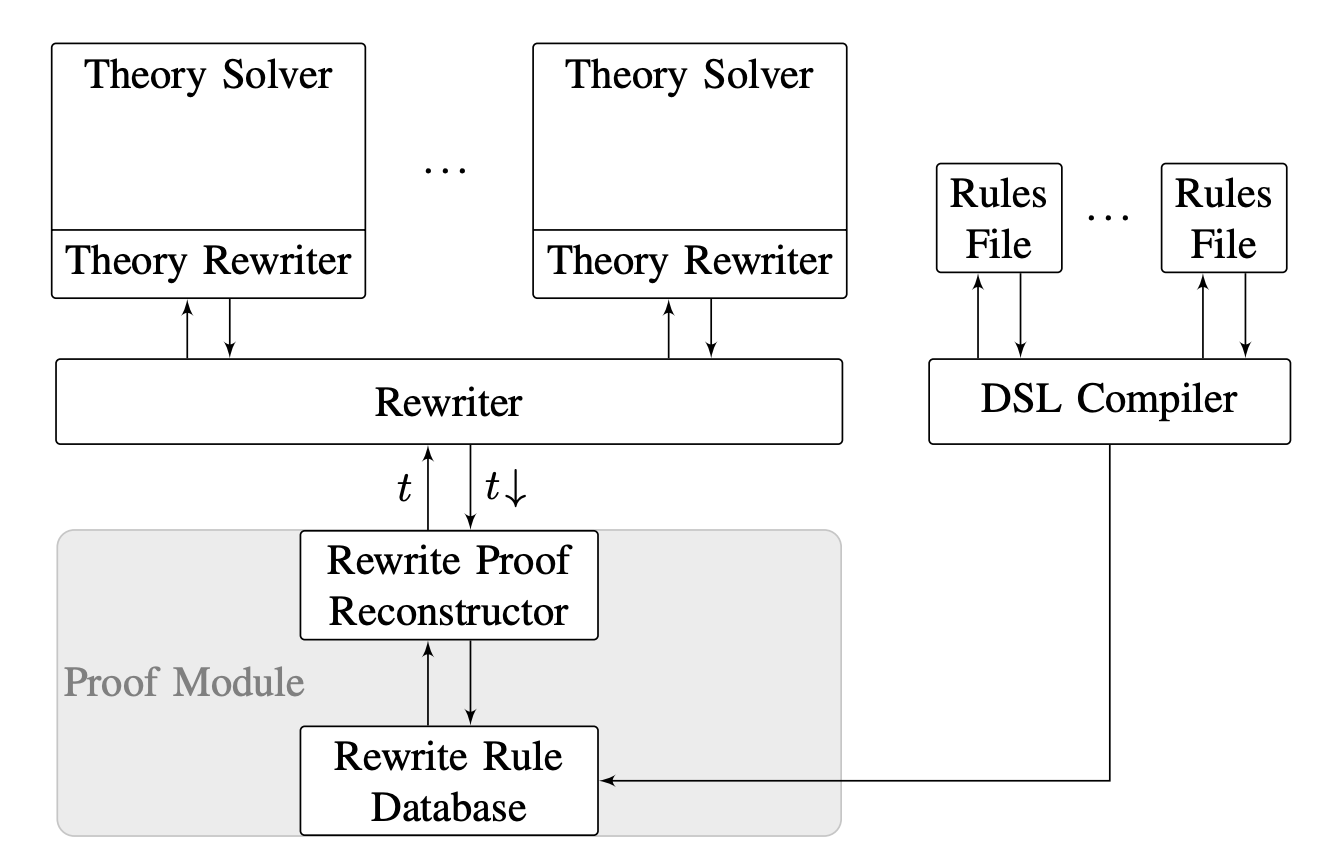
\includegraphics[scale=0.3]{RARE.png}
\vfill
\begin{quote}[RARE]
Schurr, HJ., et.al. Reliable Reconstruction of Fine-grained Proofs in a Proof Assistant. CADE 2021. Springer, Cham.
\end{quote}
\end{frame}

\begin{frame}[fragile]
\frametitle{Checking linear arithmetic steps}
\begin{itemize}
\item The \texttt{la\_generic} rule models linear arithmetic reasoning
\item For example, consider this \texttt{la\_generic} step:
\begin{minted}[allowlocal, autogobble, fontsize=\footnotesize, frame=single]{smt.py:CustomLexer}
(step t1
    (cl (<= (- x) 1) (<= (+ (* 2 x) (* (- 3) y)) 2) (<= y (- 1)))
    :rule la_generic :args (2 1 3))
\end{minted}
\item It introduces the following tautology:
$$(-x \leq 1) \lor (2x - 3y \leq 2) \lor (y \leq -1)$$
\end{itemize}
\end{frame}

\begin{frame}[fragile]
\frametitle{Checking linear arithmetic steps}
\begin{itemize}
\begin{minted}[allowlocal, autogobble, fontsize=\footnotesize, frame=single, escapeinside=||]{smt.py:CustomLexer}
(step t1
    (cl (<= (- x) 1) (<= (+ (* 2 x) (* (- 3) y)) 2) (<= y (- 1)))
    :rule la_generic |\chighlight{yellow!60}{:args (2 1 3}|))
\end{minted}
\item Checking that this clause is true is equivalent to proving that its
negation, the following three inequalites, are contradictory
\item Since \texttt{la\_generic} steps provide the needed coefficients as
    arguments, checking them is simple
\item Computing $2 \cdot (a) + 1 \cdot (b) + 3 \cdot (c)$, we get $0 > 1$,
    so the step must be true
\end{itemize}
\end{frame}

\begin{frame}[fragile]
\frametitle{Checking linear arithmetic steps}
\begin{itemize}
\item The \texttt{lia\_generic} rule is very similar to
\texttt{la\_generic}, but it does not provide the coefficients as arguments:
\begin{minted}[allowlocal, autogobble, fontsize=\footnotesize, frame=single]{smt.py:CustomLexer}
(step t1
    (cl (<= (- x) 1) (<= (+ (* 2 x) (* (- 3) y)) 2) (<= y (- 1)))
    :rule lia_generic)
\end{minted}
\item In this case, the checker would need to search for the coefficients,
which is an NP-hard problem
\item Instead, occurences of this rule are not checked, and are considered
holes by Carcara
\end{itemize}
\end{frame}

\begin{frame}{Proposal for reconstructing arithmetic steps}
\begin{figure}
    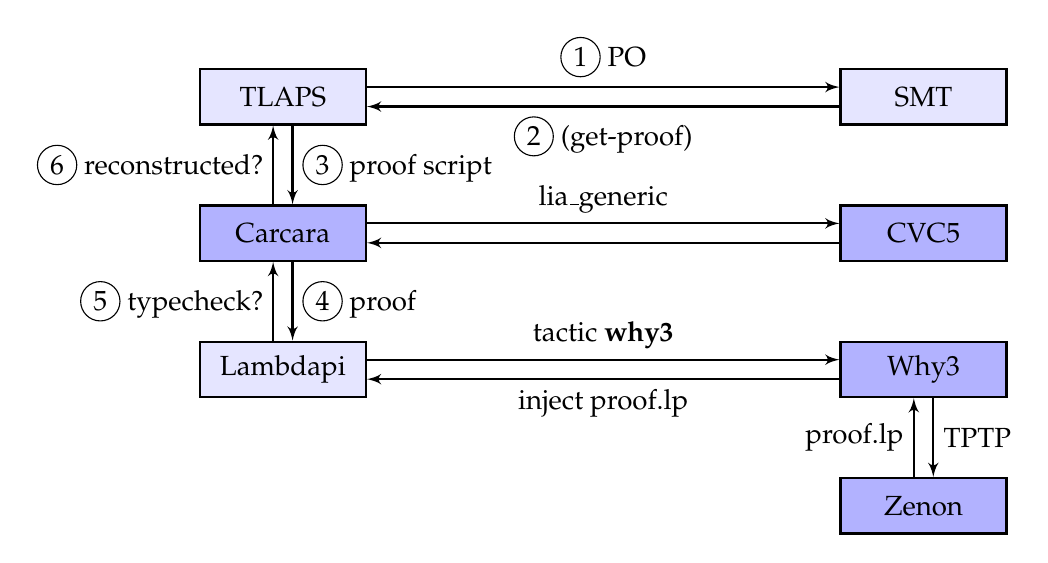
\begin{tikzpicture}[
        node distance=1cm and 6cm,
        >=latex',
        auto,
        thick,
        service/.style={draw, fill=blue!10,  minimum height=2em, minimum width=6em},
        newservice/.style={draw, fill=blue!30,  minimum height=2em, minimum width=6em},
    ]
        \node[service] (tlaps) {TLAPS};
        \node[service, right = of tlaps] (smt) {SMT};
        \node[newservice, below = of tlaps] (carcara) {Carcara};
        \node[newservice, right = of carcara] (cvc5) {CVC5};
        \node[service, below = of carcara] (lp) {Lambdapi};
        \node[newservice, right = of lp, node distance=0.5cm] (why) {Why3};
        \node[newservice, below = of why, node distance=0.5cm ] (zenon) {Zenon};
    
    \path[->, shift left=.75ex]
        (tlaps) edge node {\circled{1} PO}   (smt)
        (smt) edge   node {\circled{2} (get-proof)} (tlaps)
        (tlaps) edge node {\circled{3} proof script} (carcara)
        (carcara) edge node {\circled{6} reconstructed?} (tlaps)
        (carcara) edge  node {\circled{4} proof} (lp)
        (lp) edge  node {\circled{5} typecheck?} (carcara)
        (carcara) edge node {lia\_generic}   (cvc5)
        (cvc5) edge node {}   (carcara)
        (lp) edge node {tactic \textbf{why3}} (why)
        (why) edge node {inject proof.lp} (lp)
        (why) edge node {TPTP} (zenon)
        (zenon) edge node {proof.lp} (why)
        ;
        \end{tikzpicture}
\end{figure}
\end{frame}

\section{Future perspectives}

\begin{frame}{Future perspectives}
    \begin{itemize}
        \item Finish to validate \textit{Allocator.tla},
        \item add support for arithmetic steps,
        \item support for simplicifation steps,
        \item connect lambdapi $\text{TLA}^+$ encoding ($\textit{tla-lambdapi}$) with $\text{TLA}^+$ SMT encoding,
        \item link Event-B encoding with tla-lambdapi (shared set theory library).
    \end{itemize}
\end{frame}

\end{document}
